\documentclass[preview=true, tikz]{standalone}
% Tikz Setup
\usetikzlibrary{shapes.geometric, arrows}
\usetikzlibrary{positioning}

\begin{document}
    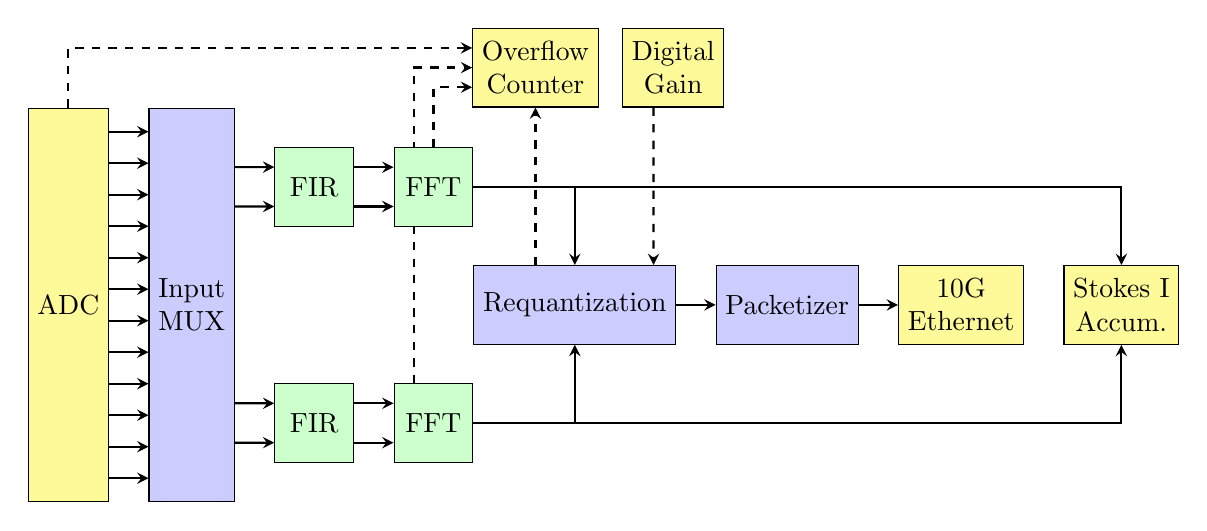
\begin{tikzpicture}
        \node[draw,minimum width=1cm,minimum height=5cm,align=center,fill=yellow!40] (adc) at (0,0) {ADC};
        \node[draw,minimum width=1cm,minimum height=5cm, right=of adc, align=center,fill=blue!20,xshift=-0.5cm] (mux) {Input\\MUX};
        \node[draw,minimum width=1cm,minimum height=1cm, right=of mux, align=center, yshift=1.5cm,fill=green!20,xshift=-0.5cm] (fir1) {FIR};
        \node[draw,minimum width=1cm,minimum height=1cm, right=of mux, align=center, yshift=-1.5cm,fill=green!20,xshift=-0.5cm] (fir2) {FIR};
        \node[draw,minimum width=1cm,minimum height=1cm, right=of fir1, align=center,fill=green!20,xshift=-0.5cm] (fft1) {FFT};
        \node[draw,minimum width=1cm,minimum height=1cm, right=of fir2, align=center,fill=green!20,xshift=-0.5cm] (fft2) {FFT};
        \node[draw,minimum width=1cm,minimum height=1cm, right=of fft1, align=center, yshift=-1.5cm, fill=blue!20,xshift=-1cm] (requant) {Requantization};
        \node[draw,minimum width=1cm,minimum height=1cm, right=of requant, align=center,fill=blue!20,xshift=-0.5cm] (pkt) {Packetizer};
        \node[draw,minimum width=1cm,minimum height=1cm, right=of pkt, align=center,fill=yellow!40,xshift=-0.5cm] (eth) {10G \\Ethernet};
        \node[draw, above=of requant,fill=yellow!40,align=center,yshift=1cm,minimum width=1cm,minimum height=1cm,xshift=-0.5cm] (ovfl) {Overflow \\ Counter};
        \node[draw, right=of eth,fill=yellow!40,align=center,xshift=-0.5cm,minimum width=1cm,minimum height=1cm] (vacc) {Stokes I \\ Accum.};
        \node[draw, above=of requant,fill=yellow!40,align=center,xshift=1.25cm,minimum width=1cm,minimum height=1cm,yshift=1cm] (gain) {Digital\\Gain};


         \draw[-stealth, thick] ([yshift=-.25cm]fir1.east) -- ([yshift=-.25cm]fft1.west);
         \draw[-stealth, thick] ([yshift=.25cm]fir1.east) -- ([yshift=.25cm]fft1.west);

         \draw[-stealth, thick] ([yshift=.25cm]fir2.east) -- ([yshift=.25cm]fft2.west);
         \draw[-stealth, thick] ([yshift=-.25cm]fir2.east) -- ([yshift=-.25cm]fft2.west);

         \draw[-stealth, thick] (fft1) -| (requant);
         \draw[-stealth, thick] (fft2) -| (requant);

         \draw[-stealth, thick] (requant) -- (pkt);
         \draw[-stealth, thick] (pkt) -- (eth);

         \draw[-stealth, thick, dashed] (fft1.north) |- ([yshift=-.25cm]ovfl.west);
         \draw[-stealth, thick, dashed] ([xshift=-.25cm]fft2.north) |- (ovfl.west);
         \draw[-stealth, thick, dashed] (adc.north) |- ([yshift=.25cm]ovfl.west);
         % redraw over arrow
         \node[draw,minimum width=1cm,minimum height=1cm, right=of fir1, align=center,fill=green!20,xshift=-0.5cm] (fft1) {FFT};

         \draw[-stealth, thick, dashed] ([xshift=-.5cm]requant.north) -- (ovfl.south);

         \draw[-stealth, thick] (fft1) -| (vacc.north);
         \draw[-stealth, thick] (fft2) -| (vacc.south);
         % redraw over arrow
        \node[draw,minimum width=1cm,minimum height=1cm, right=of requant, align=center,fill=blue!20,xshift=-0.5cm] (pkt) {Packetizer};

        \draw[-stealth, thick, dashed] ([xshift=-0.25cm]gain.south) -- ([xshift=1cm]requant.north);

         %% Input
         \draw[-stealth, thick] ([yshift=2.2cm]adc.east) -- ([yshift=2.2cm]mux.west);
         \draw[-stealth, thick] ([yshift=1.8cm]adc.east) -- ([yshift=1.8cm]mux.west);
         \draw[-stealth, thick] ([yshift=1.4cm]adc.east) -- ([yshift=1.4cm]mux.west);
         \draw[-stealth, thick] ([yshift=1.0cm]adc.east) -- ([yshift=1.0cm]mux.west);
         \draw[-stealth, thick] ([yshift=0.6cm]adc.east) -- ([yshift=.6cm]mux.west);
         \draw[-stealth, thick] ([yshift=0.2cm]adc.east) -- ([yshift=0.2cm]mux.west);
         \draw[-stealth, thick] ([yshift=-0.2cm]adc.east) -- ([yshift=-0.2cm]mux.west);
         \draw[-stealth, thick] ([yshift=-0.6cm]adc.east) -- ([yshift=-.6cm]mux.west);
         \draw[-stealth, thick] ([yshift=-1.0cm]adc.east) -- ([yshift=-1.0cm]mux.west);
         \draw[-stealth, thick] ([yshift=-1.4cm]adc.east) -- ([yshift=-1.4cm]mux.west);
         \draw[-stealth, thick] ([yshift=-1.8cm]adc.east) -- ([yshift=-1.8cm]mux.west);
         \draw[-stealth, thick] ([yshift=-2.2cm]adc.east) -- ([yshift=-2.2cm]mux.west);

        \draw[-stealth, thick] ([yshift=1.25cm]mux.east) -- ([yshift=-.25cm]fir1.west);
        \draw[-stealth, thick] ([yshift=1.75cm]mux.east) -- ([yshift=.25cm]fir1.west);

        \draw[-stealth, thick] ([yshift=-1.75cm]mux.east) -- ([yshift=-.25cm]fir2.west);
        \draw[-stealth, thick] ([yshift=-1.25cm]mux.east) -- ([yshift=.25cm]fir2.west);
         
    \end{tikzpicture}
\end{document}